\documentclass[12pt]{extarticle}
%Some packages I commonly use.
\usepackage[english]{babel}
\usepackage{graphicx}
\usepackage{framed}
\usepackage[normalem]{ulem}
\usepackage{amsmath}
\usepackage{amsthm}
\usepackage{amssymb}
\usepackage{amsfonts}
\usepackage{enumerate}
\usepackage[utf8]{inputenc}
\usepackage{float}
\usepackage[top=1 in,bottom=1in, left=1 in, right=1 in]{geometry}

%A bunch of definitions that make my life easier
\newcommand{\matlab}{{\sc Matlab} }
\newcommand{\cvec}[1]{{\mathbf #1}}
\newcommand{\rvec}[1]{\vec{\mathbf #1}}
\newcommand{\ihat}{\hat{\textbf{\i}}}
\newcommand{\jhat}{\hat{\textbf{\j}}}
\newcommand{\khat}{\hat{\textbf{k}}}
\newcommand{\minor}{{\rm minor}}
\newcommand{\trace}{{\rm trace}}
\newcommand{\spn}{{\rm Span}}
\newcommand{\rem}{{\rm rem}}
\newcommand{\ran}{{\rm range}}
\newcommand{\range}{{\rm range}}
\newcommand{\mdiv}{{\rm div}}
\newcommand{\proj}{{\rm proj}}
\newcommand{\R}{\mathbb{R}}
\newcommand{\N}{\mathbb{N}}
\newcommand{\Q}{\mathbb{Q}}
\newcommand{\Z}{\mathbb{Z}}
\newcommand{\<}{\langle}
\renewcommand{\>}{\rangle}
\renewcommand{\emptyset}{\varnothing}
\newcommand{\attn}[1]{\textbf{#1}}
\theoremstyle{definition}
\newtheorem{theorem}{Theorem}
\newtheorem{corollary}{Corollary}
\newtheorem*{definition}{Definition}
\newtheorem*{example}{Example}
\newtheorem*{note}{Note}
\newtheorem{exercise}{Exercise}
\newcommand{\bproof}{\bigskip {\bf Proof. }}
\newcommand{\eproof}{\hfill\qedsymbol}
\newcommand{\Disp}{\displaystyle}
\newcommand{\qe}{\hfill\(\bigtriangledown\)}
\setlength{\columnseprule}{1 pt}


\title{Lentes Delgadas Esféricas}
\author{Felipe Salvador}
\date{Abril 2019}

\begin{document}

\maketitle
Depois de vermos refração, vamos estudar uma aplicação muito interessante que são as lentes. As lentes são objetos transparentes de materiais diversos, a qual a luz é refratada quando entra e quando sai da lente. No nosso caso, iremos trabalhar com lentes esféricas, que possuem semelhanças com os espelhos esféricos (além do formato). Além disso, iremos trabalhar com lentes delgadas, ou seja, a espessura da lente é muito menor que a distância do foco, do centro de curvatura e do objeto.
Há 2 tipos de lente que iremos tratar:
\begin{enumerate}
\item 
\textbf{Lentes Convergentes:}
São lentes que quando raios de luz incidem perpendicularmente ao eixo central da lente, esses raios emergem da lente se aproximando entre si (convergindo para um ponto). Há um ponto em que todos os raios emergidos de luz se cruzam, a qual chamamos de foco da lente. \textbf{Para as lentes convergentes, a distância focal é positiva. ($f > 0$)}

\item
\textbf{Lentes Divergentes:}
São lentes que quando raios de luz incidem perpendicularmente ao eixo central da lente, esses raios emergem da lente se afastando
entre si (divergindo). Podemos pensar que os raios emergidos são originados de um ponto, a qual é o foco da lente. \textbf{Para as lentes, a distância focal é negativa ($f < 0$)}.
%como você falou primeiro das convergentes e depois das divergentes, sugiro inverter a ordem das duas lentes na figura. A questão de o que é positivo e o que é negativo está bem explicado em um livro que eu tenho de física do colegial, me lembre de te mandar foto desse livro.
\begin{figure}[H]
    \centering
    
\includegraphics[width=250]{imagens/lentes_delgadas.png}
    \caption{Representação de como funciona as lentes. A esquerda, é a lente divergente,perceba que após passar pela lente, os raios de luz se afastam entre si. \textbf{Com isso,podemos pensar que os raios emergidos da lente são “originados” de um ponto a qual é o foco da lente}. A direita, é a lente convergente, perceba que após passar pela lente, \textbf{os raios de luz convergem (aproximam-se) até se encontrarem, todos, num ponto que é o foco da lente}} .
    \label{fig:convergente}
\end{figure}
\end{enumerate}
%cuidado com vírgulas e pontos. Sempre colocar espaço depois deles, para deixar o texto mais leve.

A semelhança entre lentes e espelhos esféricos se dá, no caso convergente,quando os raios de luz, após serem refletidos/ refratados, se encontrarem num ponto e, no caso divergente, quando os raios de luz, após serem refletidos/ refratados, se afastam entre si, se comportando como se \textit{os raios fossem originados de um ponto} \footnote{O comportamento dos raios de luz emergidos de uma lente divergente é o mesmo do  que dos raios emitidos por uma fonte de luz pontual. Ex: Ver uma lâmpada a uma distãncia muito grande}.

Além disso, lentes e espelhos possuem focos (‘$F$’) e distâncias focais (‘$f$’), centros de curvatura (‘$C$’) e raios de curvatura (‘$r$’). Vimos em espelhos esféricos a relação entre distância focal e raio de curvatura. Ela também vale para lentes esféricas:
\begin{equation} \label{eq:1}
    r= 2f
\end{equation}

Da mesma forma, as relações de aumento linear (‘$A$’) e que envolve a distância focal (‘$f$’), a distância do objeto (‘$p$’) e a distância da imagem (‘$p’$‘) também são válidas para lentes:
\begin{equation} \label{eq:2}
   A= \frac{i}{o} = \frac{-p'}{p} = \frac{f}{f-p} 
\end{equation}
\begin{equation} \label{eq:3}
    \frac{1}{f}=\frac{1}{p}+ \frac{1}{p'}
\end{equation}
\begin{equation} \label{eq:4}
    \frac{1}{f} = (n-1)(\frac{1}{R_{1}} - \frac{1}{R_{2}})
\end{equation}

Essa equação (\ref{eq:4}) descreve como a distância focal ('$f$') é definida, uma vez que ela depende do material da lente e de '$R_{1} $' e '$R_{2}$' que são os raios de curvatura que compõe a lente.

\begin{figure} [H]
    \centering
    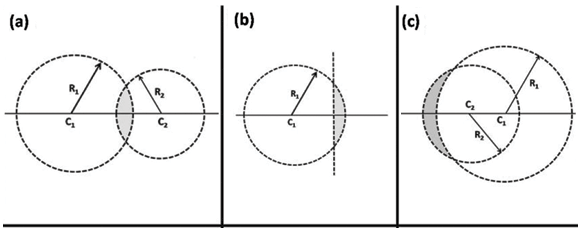
\includegraphics{imagens/raios_de_curvatura.png}
    \caption{Esquema de construção das lentes, relacionando aos raios de curvatura ('$R_{1}$' e '$R_{2}$'). A parte em cinza é a lente. Quando $R_{1}$ ou $R_{2}$ vão ao infinito ($R_{1}$ ou $R_{2}$ $\to\infty$), uma face da lente é plana. \cite{scielo}} 
    \label{fig:constr_lente}
\end{figure}

Perceba que se $R_{1}$ $>$ $R_{2}$, então $\frac{1}{R_{1}} < \frac{1}{R_{2}}$. Ou seja, pela equação (\ref{eq:4}), $\frac{1}{f}$ será \textbf{negativo}, logo a lente será \textbf{divergente}.

Se $R_{1}$ $<$ $R_{2}$, então $\frac{1}{R_{1}} > \frac{1}{R_{2}}$. Ou seja, pela equação (\ref{eq:4}), $\frac{1}{f}$ será \textbf{positivo}, logo a lente será \textbf{convergente}.

%acho que seria legal discutir em detalhe a equação (4), indicando o que são esses raios, o que acontece se um deles for 'infinito' (face plana), porque um tem sinal de menos e outro não e por aí vai.
\section{Associação de Lentes e Vergência}
\subsection{Associação de Lentes}

Para lentes, é possível combinar várias lentes e produzir efeitos diferentes. Mais ainda, ao invés de colocar várias lentes, é possível com uma lente somente obter o efeito desejado. Para isso, existe uma fórmula que é:
\begin{equation} \label{eq:5}
    \frac{1}{f_{eq}}= \frac{1}{f_{1}} + \frac{1}{f_{2}} + ...
\end{equation}
Em que $f_{eq}$ é a distância focal da lente equivalente que produz o mesmo efeito que a associação das outras lentes e $f_{1}, f_{2},...$ são as distâncias focais das lentes associadas.

\subsection{Vergência}

Existe uma quantidade chamada \textbf{Vergência}, que é definida da seguinte forma:
\begin{equation} \label{eq:6}
    V= \frac{1}{f}
\end{equation}
A unidade dessa grandeza é chamada de \textbf{dioptrias (di)} e é:
\begin{equation} \label{eq:7}
    [V]= di = \frac{1}{m} = m^{-1}
\end{equation}
%achei o portanto terminando este parágrafo esquisito. Parece que ele está amarrando a frase "(...) com distância focal de 0.20m" com os dois tópicos que vêm depois. Acho que seria legal falar da questão do sinal antes de falar de unidade e dos oftalmologistas.
Perceba que \textbf{quanto maior $f$ é, menor $V$ é}. Portanto:
\begin{itemize}
    \item 
    Para lentes convergentes ($f>0$), a vergência é positiva ($V>0$)
    \item
    Para lentes divergentes ($f<0$), a vergência é negativa ($V<0$)
\end{itemize}

Normalmente, a vergência é usada por oftalmologistas quando receitam óculos/lentes de contato. Um óculos para míopes que tem $5 di$, possui um par de lentes com distância focal de $0.20 m$.

\section{Casos da formação de imagens por lentes}

Dependendo de onde você coloca o seu objeto e de qual lente, a imagem formada será diferente. Ao todo, temos 6 casos: 5 para lentes convergentes e 1 para lentes divergentes. Mas antes de avaliarmos esses casos, iremos padronizar os \textbf{raios principais}, que são os raios de luz que passam pela ponta do objeto e carregam a
informação de onde está a imagem.

\textbf{Método}: Para descobrir onde está a imagem, iremos precisar de 2 raios de luz, que passam pelo topo do nosso objeto, fazendo caminhos diferentes. Onde esses raios se encontram é onde está o topo da imagem do objeto. Ficará mais claro nos desenhos
nos casos. Há 3 raios principais que iremos usar:

\begin{enumerate}
    \item 
    Um raio que vem paralelo ao eixo principal, passa pela lente e vai em direção ao foco;
    \item
    Um raio que passa pelo foco, passa pela lente e sai paralelo ao eixo principal;
    \item
    Um raio que passa no cruzamento do eixo principal e da lente (centro ótico) e não muda de direção (não sofre desvio).
%existe também uma quarta regra, relacionada a raios que venham alinhados com o centro de curvatura, mas fica a seu critério colocar.
\end{enumerate}
%acho legal sugerir que saibam bem essas regras de raios e também sugerir que saibam fazer esses desenhos. No meu colegial eu, fazia esses desenhos se eu precisasse responder sobre esse assunto, esboços rápidos, mesmo, com uma precisão mínima necessária, e graças a isso eu nunca precisei decorar os casos de lentes.

O mais importante num estudo geométrico das lentes, é saber desenhar esse raios principais. Os desenhos a seguir são todos mostrando caso a caso, como a imagem muda dependendo da posição do objeto e da lente usada. Não é necessário decorar caso a caso, basta saber desenhar os raios principais que qualquer exercício que necessite o desenho será feito facilmente.

\subsection{Caso de um objeto atrás do centro de curvatura para lente convergente}
%acho importante, nessas imagens, substituir o 2F por C, para deixar claro que é ali o centro de curvatura. AAAh e outra coisa: para lentes, não se usa o termo Centro de Curvatura (C), e sim Antiprincipal (A). Pelo menos, eu aprendi assim.
\begin{figure}[H]
    \centering
    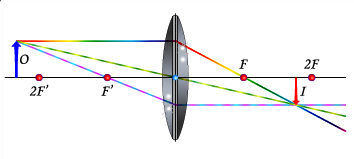
\includegraphics[width=\linewidth]{imagens/objeto-antes-ponto-antiprincipal.jpg}
    \caption{Esquema dos raios principais para um objeto atrás do centro de curvatura da lente.\cite{mundoeducacao}}
    \label{fig:obj_antes_centro}
\end{figure}

Perceba que a imagem é \textbf{real} (está do outro lado da lente), \textbf{invertida} (está para baixo do eixo principal) e \textbf{menor}. Exemplos de aplicação são o olho humano e câmaras fotográficas e filmadoras.

\subsection{Caso de um objeto no centro de curvatura para lente convergente}

\begin{figure}[H]
    \centering
    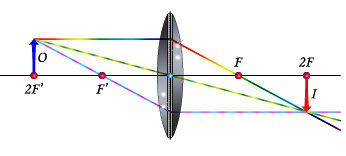
\includegraphics[width=\linewidth]{imagens/objeto-sobre-ponto-antiprincipal.jpg}
    \caption{Esquema dos raios principais para um objeto no centro de curvatura da lente. \cite{mundoeducacao}}
    \label{fig:obj_no_centro}
\end{figure}

Perceba que a imagem é \textbf{real} (está do outro lado da lente), \textbf{invertida} (está para baixo do eixo principal) e \textbf{igual}. O exemplo de aplicação é a máquina de fotocopias (\textit{xerox}).

\subsection{Caso de um objeto entre centro de curvatura e o foco para lente convergente}

\begin{figure}[H]
    \centering
    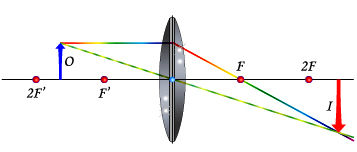
\includegraphics[width=\linewidth]{imagens/objeto-entre-ponto-antiprincipal-foco.jpg}
    \caption{Esquema dos raios principais para um objeto entre centro de curvatura e o foco da lente. \cite{mundoeducacao}}
    \label{fig:obj_entre_centro_foco}
\end{figure}

Perceba que a imagem é \textbf{real} (está do outro lado da lente), \textbf{invertida} (está para baixo do eixo principal) e \textbf{maior}. Um exemplo de aplicação é o projetor de imagens.

\subsection{Caso de um objeto no foco para lente convergente}

\begin{figure}[H]
    \centering
    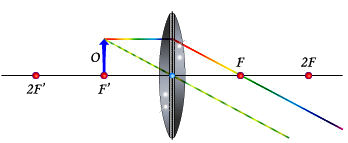
\includegraphics[width=\linewidth]{imagens/objeto-sobre-foco.jpg}
    \caption{Esquema dos raios principais para um objeto no foco da lente. \cite{mundoeducacao}}
    \label{fig:obj_no_foco}
\end{figure}

Perceba que não é formada imagem (os raios que saem da lente são paralelos entre si). Uma outra interpretação é que a imagem é formada \textit{no infinito} (imagem imprópria). Porém, não gosto dessa interpretação, pois não é possivel enxergar essa imagem num anteparo.
%dizem também que é uma imagem imprópria.
\subsection{Caso de um objeto na frente do foco para lente convergente}

\begin{figure}[H]
    \centering
    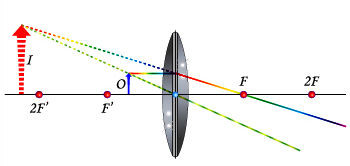
\includegraphics[width=\linewidth]{imagens/objeto-entre-foco-centro-optico.jpg}
    \caption{Esquema dos raios principais para um objeto na frente do foco da lente. \cite{mundoeducacao}}
    \label{fig:obj_a_frente_foco}
\end{figure}

Perceba que a imagem é \textbf{virtual} (está do mesmo lado da lente), \textbf{direita} (está para cima do eixo principal) e \textbf{maior}. Exemplos de aplicação são a lupa e o óculos de leitura.

\subsection{Caso geral de uma lente divergente}

\begin{figure}[H]
    \centering
    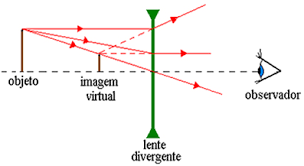
\includegraphics[width=\linewidth]{imagens/lente_divergente.png}
    \caption{Esquema dos raios principais para um objeto a frente de uma lente divergente. \cite{alunosonline}}
    \label{fig:obj_divergente}
\end{figure}

Perceba que a imagem é \textbf{virtual} (está do mesmo lado da lente), \textbf{direita} (está para cima do eixo principal) e \textbf{menor}. Um exemplo de aplicação é óculos para miopia (não enxerga de longe).

\section{Formatos das Lentes}
%existe um critério para saber qual nome você fala antes: ver qual raio é maior. Na concavo-convexa, por exemplo, o raio da face côncava é maior. A palavra plano sempre vem antes porque implica num "raio infinito".
Vimos que temos 2 tipos de lentes, convergentes e divergentes. Mas elas podem ter formatos diferentes e os vestibulares gostam de falar de lentes falando dos seus formatos.

É muito importante é saber esses nomes, porque muitas vezes o exercício não diz se uma lente é convergente, mas fala que a lente é plano-convexa e você precisa saber quais formatos de lente provocam convergência ou divergência.

Em geral, há 6 formatos de lentes que trabalhamos:

\begin{figure} [H]
    \centering
    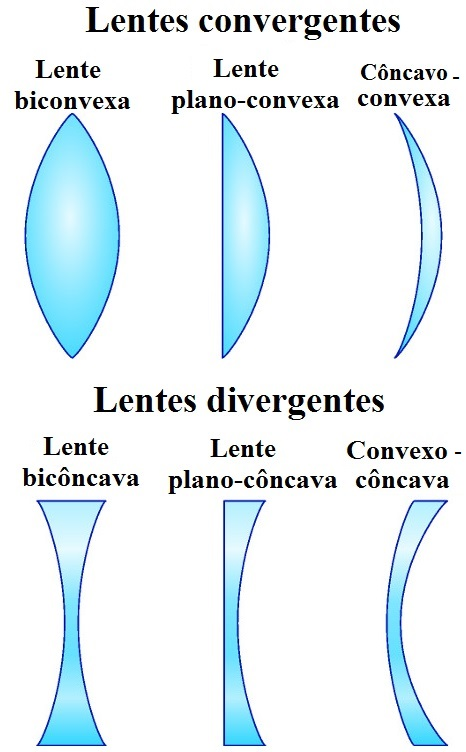
\includegraphics[width = 200]{imagens/tipos_de_lentes.jpg}
    \caption{Formato das lentes para cada tipo de lente \cite{brasilescola}}
    \label{fig:formato_lentes}
\end{figure}

\section{Situações em que $n_{lente}< n_{meio}$}

Até aqui, estamos falando de lentes imersas em meios que tem o índice de refração $n$ menor que o da lente ($n_{lente} > n_{meio}$).

Porém, podemos ter exercícios que abordem o contrário: o meio possui índice de refração maior que o da lente ($n_{lente} < n_{meio}$). Isso acontece, por exemplo, tiver uma bolha de ar, funcionando como uma lente, num tanque de água. Nesses casos, o que a lente faz é o \textbf{oposto que ela faria no caso anterior}, ou seja:
\begin{itemize}
    \item 
    Se a lente era \textbf{convergente} quando $n_{lente} > n_{meio}$ , agora ela é uma lente \textbf{divergente} quando $n_{lente} < n_{meio}$;
    \item
    Se a lente era \textbf{divergente} quando $n_{lente} > n_{meio}$ , agora ela é uma lente \textbf{convergente} quando $n_{lente} < n_{meio}$.
\end{itemize}

\begin{figure}[H]
    \centering
    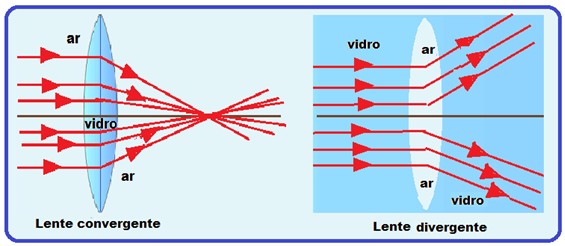
\includegraphics{imagens/casos_para_n_diferente.png}
    \caption{Imagem representativa dos dois casos. Quando trocado os papéis entre meio e a lente, a lente troca de papel também \cite{fisicaevestibular}}
    \label{fig:casos_p/_n_diferente}
\end{figure}

\section{Exemplos}

\begin{enumerate}
%exemplo 1%
    \item
    Um objeto está a 60 cm de uma lente biconvexa que possuem foco em 20 cm. Com base nestas informações, calcule:
    \begin{enumerate}
        \item 
        A distância da imagem formada até a lente.
        \item
        Caracterize a imagem. (Descubra o aumento linear (A) e faça desenho)
    \end{enumerate}
    
    \textit{Respostas:}
    
    \begin{enumerate}
%item a da resolução do exemplo 
        \item 
        Como a lente é biconvexa, a lente é convergente. (Quando o enunciado não fala nada, suponha que o comportamento da lente é o usual). Então, a distância focal tem que ser positiva. Vamos usar a equação \ref{eq:3}, sabendo que o enunciado nos deu a distância focal, $f = 20 cm$, e a distância do objeto à lente, $p = 60 cm$. Aplicando na equação \ref{eq:3}, temos que:
        
        \begin{align*}
        \frac{1}{20}= \frac{1}{60} + \frac{1}{p'}
        \end{align*}
        
        \begin{align*}
        \frac{1}{p'}= \frac{6-2}{120} \implies p'=30 cm
        \end{align*}
        
%item b da resolução do exemplo  
        \item
        Com $p'$ determinado, podemos usar a equação \ref{eq:2} para determinar o aumento linear $A$:
        \begin{align*}
            A = \frac{-p'}{p}= - \frac{30}{60} \implies A = -0.5
        \end{align*}
        
        Como $A$ = $\frac{i}{o}$= -0.5, sabemos que a imagem é invertida (o objeto $o$ sempre possui tamanho positivo) e tem metade do tamanho do objeto. Logo, o desenho ficará:
        
        \begin{figure} [H]
            \centering
            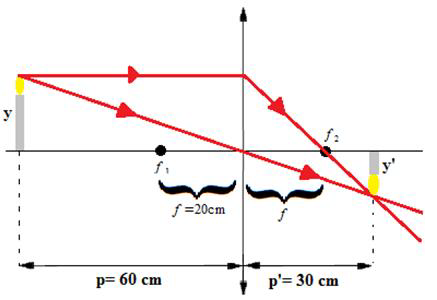
\includegraphics{imagens/imagem_ex_1_lentes.png}
            \caption{Desenho geométrico de como fica o exemplo}
            \label{fig:ex1}
        \end{figure}
    \end{enumerate}

%exemplo 2
    \item
    Uma lente cujas faces tem 20 e 40 cm de raios de curvatura está imersa no ar. Sendo 1,5 o índice de refração do vidro, calcule:
    \begin{enumerate}
        \item 
        Sua vergência e o tipo de lente.
        \item
        Sua distância focal.
    \end{enumerate}
    
    \textit{Respostas:}
    \begin{enumerate}
    
%resolucao item a
        \item 
        
        Sabemos pela equação (\ref{eq:6}) que: 
        \begin{align*}
            V=\frac{1}{f}
        \end{align*}
        
        E pela equação (\ref{eq:4}) que: 
        \begin{align*}
            \frac{1}{f} = (n-1)(\frac{1}{R_{1}} - \frac{1}{R_{2}})
        \end{align*}
        
        Juntando (\ref{eq:6}) em (\ref{eq:4}):
        \begin{align*}
            V = (n-1)(\frac{1}{R_{1}} - \frac{1}{R_{2}})
        \end{align*}
        
        Com os dados do problema, temos que \footnote{Eu sou obrigado a transformar os dados em $cm$ para $m$ para poder expressar a vergência em $di$}:
        \begin{align*}
            V = (1.5-1)(\frac{1}{0.2} - \frac{1}{0.4}) = 0.5(\frac{2-1}{0.4}) = \frac{0.5}{0.4} \implies V = 1.25 di
        \end{align*}
        Como $V>0$, a lente é convergente.
        
%resolucao item b
        \item
        Pela equação (\ref{eq:6}) sabemos que: $V= \frac{1}{f}$ e sabemos que $V=1.25 di$, então:
        
        \begin{align*}
            1.25 = \frac{1}{f} \implies f = \frac{1}{1.25} = 0.80 m
        \end{align*}
        \begin{align*}
            f = 0.80 m = 80 cm
        \end{align*}
    \end{enumerate}

\end{enumerate}

\begin{thebibliography}{9}




\bibitem{scielo}
Pionório, N., Rodrigues Jr, J.J. e Bertuola, A.C..

\textit{ Correções da aberração cromática no contexto da óptica geométrica. Revista Brasileira de Ensino de Física, 30(3), 3315.1-3315.10.} 
\texttt{https://dx.doi.org/10.1590/S1806-11172008000300015}

\bibitem{mundoeducacao}
Mundo Educação - Uol
\\\texttt{https://mundoeducacao.bol.uol.com.br/fisica/formacao-imagens-nas-lentes-esfericas.htm}

\bibitem{alunosonline}
Alunos Online - Uol
\\\texttt{https://alunosonline.uol.com.br/fisica/lentes-convergente-divergente.html}

\bibitem{brasilescola}
Brasil Escola
\\\texttt{https://brasilescola.uol.com.br/fisica/lentes-1.htm}

\bibitem{fisicaevestibular}
Física e Vestibular
\\\texttt{http://fisicaevestibular.com.br/novo/optica/optica-geometrica/lentes-construcao-geometrica-de-imagens}

\end{thebibliography}



\end{document}
